% This is samplepaper.tex, a sample chapter demonstrating the
% LLNCS macro package for Springer Computer Science proceedings;
% Version 2.21 of 2022/01/12
%
\documentclass[runningheads]{llncs}
%
\usepackage[T1]{fontenc}
% T1 fonts will be used to generate the final print and online PDFs,
% so please use T1 fonts in your manuscript whenever possible.
% Other font encondings may result in incorrect characters.
%
\usepackage{graphicx}
\usepackage{xcolor, soul}
% Used for displaying a sample figure. If possible, figure files should
% be included in EPS format.
%
% If you use the hyperref package, please uncomment the following two lines
% to display URLs in blue roman font according to Springer's eBook style:
%\usepackage{color}
%\renewcommand\UrlFont{\color{blue}\rmfamily}
%\urlstyle{rm}
%
%\usepackage{dsfont}
\usepackage{stmaryrd}
\usepackage{colortbl}
\usepackage{hyperref}

\usepackage{amsmath}
\DeclareMathOperator*{\argmax}{argmax}
\DeclareMathOperator*{\argmin}{argmin}
\usepackage{amssymb}

\usepackage[dvipsnames, table]{xcolor}
\usepackage{textcomp}

% Packages
\usepackage[pdf]{graphviz}
\usepackage{mathrsfs}

\newcommand*\circled[1]{\tikz[baseline=-0.1cm]{
  \node[shape=circle,draw,inner sep=0.48pt] (char) {\fontsize{7}{12}\textsf{#1}};}}

\DeclareMathAlphabet{\mathcal}{OMS}{cmsy}{m}{n}
\usepackage{cancel}
\newcommand\ccancel[2][red]{\renewcommand\CancelColor{\color{#1}}\cancel{#2}}
\newcommand{\nDownarrow}{\ensuremath{\text{ }\cancel{\Downarrow}\text{ }}}
\usepackage{centernot}

\usepackage{pgfplots, pgfplotstable}
\pgfplotsset{compat=1.7}
\usepgfplotslibrary{fillbetween}
\usetikzlibrary{patterns}
\pgfmathdeclarefunction{gauss}{2}{\pgfmathparse{1/(#2*sqrt(2*pi))*exp(-((x-#1)^2)/(2*#2^2))}}
\pgfmathdeclarefunction{nil}{1}{\pgfmathparse{0.001}}

\usepackage{arydshln}
\usepackage{adjustbox}
\usepackage{enumerate}
\usepackage{enumitem}
\usepackage{tikz-cd}
\usetikzlibrary{calc}
\usepackage{amsfonts}
%\usepackage{prooftrees}
\usepackage{bussproofs}
\renewcommand{\sectionautorefname}{\S}
\renewcommand{\subsectionautorefname}{\S}
\usepackage{float}

\usepackage{tikz-3dplot}
\usetikzlibrary{3d}
\usetikzlibrary{calligraphy}
\newif\ifshowcellnumber
\showcellnumbertrue

\usepackage{algorithm}
\usepackage{algpseudocode}
\usepackage{algorithmicx}
\usepackage{sourcecodepro}
\usepackage{tikz-qtree}
\usepackage{amsthm}
\usepackage{bm}
\usetikzlibrary{bayesnet}
\usetikzlibrary{arrows}
\usepackage{subcaption}
\usetikzlibrary{backgrounds}
\usetikzlibrary{tikzmark}
\usetikzlibrary{hobby}

\usepackage{mwe}

\newcommand{\E}{\mathbb{E}}
\newcommand{\Var}{\mathrm{Var}}
\newcommand{\Cov}{\mathrm{Cov}}

\newcommand{\CompOrder}{\mathcal{O}}
\def\graphspace{\mathbf{G}}
\def\Uniform{\mbox{\rm Uniform}}
\def\Gaussian{\mbox{\rm Gaussian}}
\def\Bernoulli{\mbox{\rm Bernoulli}}
\def\Dirichlet{\mbox{\rm Dirichlet}}

\usepackage{mathtools}% superior to amsmath
\usepackage{tikz}
% Packages
\usepackage{listings}
\DeclareRobustCommand{\hlred}[1]{{\sethlcolor{pink}\hl{#1}}}
\usepackage{fontspec}

\setmonofont[Scale=0.8]{JetBrainsMono}[
  Contextuals={Alternate},
  Path=./font/,
  Extension = .ttf,
  UprightFont=*-Regular,
  BoldFont=*-Bold,
  ItalicFont=*-Italic,
  BoldItalicFont=*-BoldItalic
]

\usepackage[skins,breakable,listings]{tcolorbox}

\lstdefinelanguage{kotlin}{
  comment=[l]{//},
  commentstyle={\color{gray}\ttfamily},
  emph={delegate, filter, firstOrNull, forEach, it, lazy, mapNotNull, println, repeat, assert, with, head, tail, len, return@},
  numberstyle=\noncopyable,
  identifierstyle=\color{black},
  keywords={abstract, actual, as, as?, break, by, class, companion, continue, data, do, dynamic, else, enum, expect, false, final, for, fun, get, if, import, in, infix, interface, internal, is, null, object, open, operator, override, package, private, public, return, sealed, set, super, suspend, this, throw, true, try, catch, typealias, val, var, vararg, when, where, while, tailrec, reified},
  keywordstyle={\bfseries},
  morecomment=[s]{/*}{*/},
  morestring=[b]",
  morestring=[s]{"""*}{*"""},
  ndkeywords={@Deprecated, @JvmField, @JvmName, @JvmOverloads, @JvmStatic, @JvmSynthetic, Array, Byte, Double, Float, Boolean, Int, Integer, Iterable, Long, Runnable, Short, String, int},
  ndkeywordstyle={\bfseries},
  sensitive=true,
  stringstyle={\ttfamily},
  literate={`}{{\char0}}1,
  escapeinside={(*@}{@*)}
}
\lstdefinelanguage{tidy}{
  comment=[l]{//},
  commentstyle={\color{gray}\ttfamily},
  emph={|, ->, ---},
  emphstyle={\color{red}},
  identifierstyle=\color{black},
  keywords={\|, ->, ---},
  otherkeywords={|,->},
  morekeywords={|,->},
  keywordstyle={\color{blue}\bfseries},
  morecomment=[s]{/*}{*/},
  morestring=[b]",
  morestring=[s]{"""*}{*"""},
  ndkeywords={@Deprecated, @JvmField, @JvmName, @JvmOverloads, @JvmStatic, @JvmSynthetic, Array, Byte, Double, Float, Int, Integer, Iterable, Long, Runnable, Short, String},
  ndkeywordstyle={\color{orange}\bfseries},
  sensitive=true,
  stringstyle={\color{green}\ttfamily},
  literate={`}{{\char0}}1
}

%%%%%%%%%%%%%%%%%%%%%%%%%%%%%%%%%%%%%%%%%%%
%
% Color boxes
%
%%%%%%%%%%%%%%%%%%%%%%%%%%%%%%%%%%%%%%%%%%%

\tcbset{
  enhanced jigsaw,
  breakable,
  listing only,
%  boxsep=-1pt,
%  top=-1pt,
  bottom=0.1cm,
  right=0.5cm,
  overlay first={
    \node[black!50] (S) at (frame.south) {\Large\ding{34}};
    \draw[dashed,black!50] (frame.south west) -- (S) -- (frame.south east);
  },
  overlay middle={
    \node[black!50] (S) at (frame.south) {\Large\ding{34}};
    \draw[dashed,black!50] (frame.south west) -- (S) -- (frame.south east);
    \node[black!50] (S) at (frame.north) {\Large\ding{34}};
    \draw[dashed,black!50] (frame.north west) -- (S) -- (frame.north east);
  },
  overlay last={
    \node[black!50] (S) at (frame.north) {\Large\ding{34}};
    \draw[dashed,black!50] (frame.north west) -- (S) -- (frame.north east);
  },
  before={\par\vspace{5pt}},
  after={\par\vspace{\parskip}\noindent}
}

\definecolor{slightgray}{rgb}{0.90, 0.90, 0.90}

\usepackage{soul}
\makeatletter
\def\SOUL@hlpreamble{%
  \setul{}{3.0ex}%
  \let\SOUL@stcolor\SOUL@hlcolor%
  \SOUL@stpreamble%
}
\makeatother

\newcommand{\inline}[1]{%
  \begingroup%
  \sethlcolor{slightgray}%
  \hl{\ttfamily\footnotesize #1}%
  \endgroup
}

\newcommand{\tinline}[1]{%
  \begingroup%
  \sethlcolor{slightgray}%
  \hl{\ttfamily\tiny #1}%
  \endgroup
}

\newtcblisting{halftidyinput}[1][]{%
  left skip=0.7cm,
  left=0.35cm,
  width=6cm,
%  left=-0.01cm,
  top=-0.1cm,
  bottom=-0.35cm,
  listing options={
    language=tidy,
    basicstyle=\ttfamily\small,
%numberstyle=\footnotesize,
    showstringspaces=false,
    tabsize=2,
    breaklines=true,
    numbers=none,
    inputencoding=utf8,
    escapeinside={(*@}{@*)},
    #1
  },
  underlay unbroken and first={%
    \path[draw=none] (interior.north west) rectangle node[white]{
\includegraphics[width=4mm]{../figures/tidyparse_logo.png}} ([xshift=-10mm,yshift=-7mm]interior.north west);
  }
}

\newtcblisting{wholetidyinput}[1][]{%
  left skip=0.7cm,
  left=0.35cm,
  top=0.1cm,
  middle=0mm,
  boxsep=0mm,
  listing options={
    language=tidy,
    basicstyle=\ttfamily\small,
%numberstyle=\footnotesize,
    showstringspaces=false,
    tabsize=2,
    breaklines=true,
    numbers=none,
    inputencoding=utf8,
    escapeinside={(*@}{@*)},
    #1
  },
  underlay unbroken and first={%
      \path[draw=none] (interior.north west) rectangle node[white]{
\includegraphics[width=4mm]{../figures/tidyparse_logo.png}} ([xshift=-10mm,yshift=-9mm]interior.north west);
  }
}

\definecolor{A}{RGB}{6,150,104}
\definecolor{B}{RGB}{196,74,137}
\definecolor{C}{RGB}{117,237,133}
\definecolor{D}{RGB}{246,46,243}
\definecolor{E}{RGB}{89,162,12}
\definecolor{F}{RGB}{113,12,158}
\definecolor{G}{RGB}{191,205,142}
\definecolor{H}{RGB}{51,58,158}
\definecolor{I}{RGB}{244,212,3}
\definecolor{J}{RGB}{37,36,249}
\definecolor{K}{RGB}{253,165,71}
\definecolor{L}{RGB}{27,81,29}
\colorlet{LA}{A!30}
\colorlet{LB}{B!30}
\colorlet{LC}{C!30}
\colorlet{LD}{D!30}
\colorlet{LE}{E!30}
\colorlet{LF}{F!30}
\colorlet{LG}{G!30}
\colorlet{LH}{H!30}
\colorlet{LI}{I!30}
\colorlet{LJ}{J!30}
\colorlet{LK}{K!30}
\colorlet{LL}{L!30}
\newcommand{\hiliA}[1]{%
  \colorbox{LA}{$#1$}}
\newcommand{\hiliB}[1]{%
  \colorbox{LB}{$#1$}}
\newcommand{\hiliC}[1]{%
  \colorbox{LC}{$#1$}}
\newcommand{\hiliD}[1]{%
  \colorbox{LD}{$#1$}}
\newcommand{\hiliE}[1]{%
  \colorbox{LE}{$#1$}}
\newcommand{\hiliF}[1]{%
  \colorbox{LF}{$#1$}}
\newcommand{\hiliG}[1]{%
  \colorbox{LG}{$#1$}}
\newcommand{\hiliH}[1]{%
  \colorbox{LH}{$#1$}}
\newcommand{\hiliI}[1]{%
  \colorbox{LI}{$#1$}}
\newcommand{\hiliJ}[1]{%
  \colorbox{LJ}{$#1$}}
\newcommand{\hiliK}[1]{%
  \colorbox{LK}{$#1$}}
\newcommand{\hiliL}[1]{%
  \colorbox{LL}{$#1$}}
\newcommand{\highlight}[1]{%
  \colorbox{lgray}{$#1$}}
\colorlet{lred}{red!30}
\colorlet{lorange}{orange!30}
\colorlet{lgreen}{green!30}
\colorlet{lgray}{black!15}
\colorlet{dgray}{black!75}
\DeclareRobustCommand{\hlred}[1]{{\sethlcolor{lred}\hl{#1}}}
\DeclareRobustCommand{\hlorange}[1]{{\sethlcolor{lorange}\hl{#1}}}
\DeclareRobustCommand{\hlgreen}[1]{{\sethlcolor{lgreen}\hl{#1}}}
\DeclareRobustCommand{\hlgray}[1]{{\sethlcolor{lgray}\hl{#1}}}
\DeclareRobustCommand{\caret}[1]{{\sethlcolor{dgray}\textcolor{white}{\hl{#1}}}}

\usepackage{url}
\usepackage{qtree}

\usepackage{filecontents}
\usepackage{pstricks-add}
\usepackage{emoji}
\usepackage{alltt}
\usepackage{nicematrix}
\usepackage{graphicx}
\usepackage{ulem}
\usepackage{upquote}
\tikzstyle{every picture}+=[remember picture]
\usepackage{menukeys}
\pgfplotstableread[col sep=comma,]{timings_loc.csv}\loctimings
\pgfplotstableread[col sep=comma,]{timings_unloc.csv}\unloctimings

\makeatletter
\DeclareRobustCommand{\cev}[1]{%
  {\mathpalette\do@cev{#1}}%
}
\newcommand{\do@cev}[2]{%
  \vbox{\offinterlineskip
  \sbox\z@{$\m@th#1 x$}%
  \ialign{##\cr
  \hidewidth\reflectbox{$\m@th#1\vec{}\mkern4mu$}\hidewidth\cr
  \noalign{\kern-\ht\z@}
    $\m@th#1#2$\cr
  }%
  }%
}
\makeatother

\makeatletter
\DeclareRobustCommand{\pder}[1]{%
  \@ifnextchar\bgroup{\@pder{#1}}{\@pder{}{#1}}}
\newcommand{\@pder}[2]{\frac{\partial#1}{\partial#2}}
\makeatother

\newcommand{\shup}{\shortuparrow}
\newcommand{\shri}{\shortrightarrow}
\newcommand{\shur}{\shup\hspace{-5pt}\shri}

\makeatletter
\def\squigglyred{\bgroup \markoverwith{\textcolor{red}{\lower3\p@\hbox{\sixly \char58}}}\ULon}
\makeatother

\makeatletter
\def\squigglyblu{\bgroup \markoverwith{\textcolor{blue}{\lower3\p@\hbox{\sixly \char58}}}\ULon}
\makeatother

\makeatletter
\def\squigglyora{\bgroup \markoverwith{\textcolor{orange}{\lower3\p@\hbox{\sixly \char58}}}\ULon}
\makeatother

\newcommand{\err}[1]{\smash{\squigglyred{#1}{}}}
\newcommand{\erb}[1]{\smash{\squigglyblu{#1}{}}}
\newcommand{\ero}[1]{\smash{\squigglyora{#1}{}}}
\newcommand{\stirlingii}{\genfrac{\{}{\}}{0pt}{}}

%======== Arrows =========
\newcommand{\knightarrow}{
  \tikz{
    \fill (0pt,0pt) circle [radius = 1pt];
    \fill (0pt,6pt) circle [radius = 1pt];
    \fill (6pt,0pt) circle [radius = 1pt];
    \fill (6pt,6pt) circle [radius = 1pt];
    \fill (12pt,0pt) circle [radius = 1pt];
    \fill (12pt,6pt) circle [radius = 1pt];
    \fill (6pt,0pt) circle [radius = 1pt];
    \fill (12pt,0pt) circle [radius = 1pt];
    \draw [-to] (0pt,0pt) -- (12pt,6pt);
  }
}

\newcommand{\kingarrow}{
  \tikz{
    \fill (0pt,0pt) circle [radius = 1pt];
    \fill (6pt,0pt) circle [radius = 1pt];
    \fill (0pt,6pt) circle [radius = 1pt];
    \fill (6pt,6pt) circle [radius = 1pt];
    \draw [-to] (0pt,0pt) -- (6pt,6pt);
    \draw [-to] (0pt,0pt) -- (0pt,6pt);
    \draw [-to] (0pt,0pt) -- (6pt,0pt);
  }
}

\newcommand{\duparrow}{
  \tikz{
    \fill (0pt,0pt) circle [radius = 1pt];
    \fill (0pt,6pt) circle [radius = 1pt];
    \draw [-to] (0pt,0pt) -- (0pt,6pt);
  }
}

\newcommand{\drightarrow}{
  \tikz{
    \fill (0pt,0pt) circle [radius = 1pt];
    \fill (6pt,0pt) circle [radius = 1pt];
    \draw [-to] (0pt,0pt) -- (6pt,0pt);
  }
}

\newcommand{\ddiagarrow}{
  \tikz{
    \fill (0pt,0pt) circle [radius = 1pt];
    \fill (6pt,0pt) circle [radius = 1pt];
    \fill (0pt,6pt) circle [radius = 1pt];
    \fill (6pt,6pt) circle [radius = 1pt];
    \draw [-to] (0pt,0pt) -- (6pt,6pt);
  }
}

\newcommand{\knightkingarrow}{
  \tikz{
    \fill (0pt,0pt) circle [radius = 1pt];
    \fill (0pt,6pt) circle [radius = 1pt];
    \fill (6pt,0pt) circle [radius = 1pt];
    \fill (6pt,6pt) circle [radius = 1pt];
    \fill (12pt,0pt) circle [radius = 1pt];
    \fill (12pt,6pt) circle [radius = 1pt];
    \draw [-to] (0pt,0pt) -- (6pt,6pt);
    \draw [-to] (0pt,0pt) -- (0pt,6pt);
    \draw [-to] (0pt,0pt) -- (6pt,0pt);
    \draw [-to] (0pt,0pt) -- (12pt,6pt);
  }
}

%======== Arrows =========

\usetikzlibrary{decorations.pathreplacing,automata,calc,positioning,matrix,fit,decorations.pathmorphing}

\usepackage{wrapfig}

\newcommand{\mkTrellis}[1]{
  \begin{tikzpicture}
    \def\dx{20pt}
    \def\dy{30pt}
    \newcounter{i}
    \stepcounter{i}
    \node[circle, draw, fill=black!30] (\arabic{i}) at (0,0){};
    \foreach [count=\i] \x in {2,...,#1}{
      \pgfmathsetmacro{\lox}{\x-1}%
      \pgfmathsetmacro{\loxt}{\x-3}%
      \foreach [count=\j] \xx in {-\lox,-\loxt,...,\lox}{
        \pgfmathsetmacro{\jj}{\j-1}%
        \stepcounter{i}
        \pgfmathsetmacro{\kk}{\xx-2}%
        \pgfmathsetmacro{\lbl}{\lox!/(\jj!*(\lox-\jj)!)}
        \ifnum\x<\kk
        \pgfmath\node[circle, draw]  (\arabic{i}) at (\xx*\dx, -\lox*\dy) {};
        \else
        \pgfmath\node[circle, draw, fill=black!30]  (\arabic{i}) at (\xx*\dx, -\lox*\dy) {};
        \fi
      }
    }
    \newcounter{z}
    \newcounter{xn}
    \newcounter{xnn}
    \pgfmathsetmacro{\maxx}{#1 - 1}
    \foreach \x in {1,...,\maxx}{
      \foreach \xx in {1,...,\x}{
        \stepcounter{z}
        \setcounter{xn}{\arabic{z}}
        \addtocounter{xn}{\x}
        \setcounter{xnn}{\arabic{xn}}
        \stepcounter{xnn}
        \draw [<-] (\arabic{z}) -- (\arabic{xn});
        \draw [<-] (\arabic{z}) -- (\arabic{xnn});
      }
    }
  \end{tikzpicture}
}

\newcommand{\dx}{20pt}
\newcommand{\dy}{30pt}
\newcounter{i}
\newcounter{z}
\newcounter{xn}
\newcounter{xnn}
\newcommand{\mkTrellisAppend}[1]{
  \begin{tikzpicture}
    \setcounter{i}{0}
    \setcounter{z}{0}
    \setcounter{xn}{0}
    \setcounter{xnn}{0}
    \stepcounter{i}
    \node[circle, draw] (\arabic{i}) at (0,0){};
    \foreach [count=\i] \x in {2,...,#1}{
      \pgfmathsetmacro{\lox}{\x-1}%
      \pgfmathsetmacro{\loxt}{\x-3}%
      \foreach [count=\j] \xx in {-\lox,-\loxt,...,\lox}{
        \pgfmathsetmacro{\jj}{\j-1}%
        \stepcounter{i}
        \pgfmathsetmacro{\kk}{\xx+2}%
        \pgfmathsetmacro{\lbl}{\lox!/(\jj!*(\lox-\jj)!)}
        \ifnum\x>\kk
        \pgfmath\node[circle, draw, fill=black!30]  (\arabic{i}) at (\xx*\dx, -\lox*\dy) {};
        \else
        \pgfmath\node[circle, draw]  (\arabic{i}) at (\xx*\dx, -\lox*\dy) {};
        \fi
      }
    }
    \pgfmathsetmacro{\maxx}{#1 - 1}
    \foreach \x in {1,...,\maxx}{
      \foreach \xx in {1,...,\x}{
        \stepcounter{z}
        \setcounter{xn}{\arabic{z}}
        \addtocounter{xn}{\x}
        \setcounter{xnn}{\arabic{xn}}
        \stepcounter{xnn}
        \draw [<-] (\arabic{z}) -- (\arabic{xn});
        \draw [<-] (\arabic{z}) -- (\arabic{xnn});
      }
    }
  \end{tikzpicture}
}

\newcommand{\mkTrellisInsert}[1]{
  \begin{tikzpicture}
    \setcounter{i}{0}
    \setcounter{z}{0}
    \setcounter{xn}{0}
    \setcounter{xnn}{0}
    \stepcounter{i}
    \node[circle, draw] (\arabic{i}) at (0,0){};
    \foreach [count=\i] \x in {2,...,#1}{
      \pgfmathsetmacro{\lox}{\x-1}%
      \pgfmathsetmacro{\loxt}{\x-3}%
      \foreach [count=\j] \xx in {-\lox,-\loxt,...,\lox}{
        \pgfmathsetmacro{\jj}{\j-1}%
        \stepcounter{i}
        \pgfmathsetmacro{\mp}{\xx+#1}%
        \pgfmathsetmacro{\mq}{\xx+\x}%
        \pgfmathsetmacro{\lbl}{\lox!/(\jj!*(\lox-\jj)!)}
        \ifnum\x>\mp
        \pgfmath\node[circle, draw, fill=black!30]  (\arabic{i}) at (\xx*\dx, -\lox*\dy) {};
        \else
        \ifnum#1<\mq
        \pgfmath\node[circle, draw, fill=black!30]  (\arabic{i}) at (\xx*\dx, -\lox*\dy) {};
        \else
        \pgfmath\node[circle, draw]  (\arabic{i}) at (\xx*\dx, -\lox*\dy) {};
        \fi
        \fi

      }
    }
    \pgfmathsetmacro{\maxx}{#1 - 1}
    \foreach \x in {1,...,\maxx}{
      \foreach \xx in {1,...,\x}{
        \stepcounter{z}
        \setcounter{xn}{\arabic{z}}
        \addtocounter{xn}{\x}
        \setcounter{xnn}{\arabic{xn}}
        \stepcounter{xnn}
        \draw [<-] (\arabic{z}) -- (\arabic{xn});
        \draw [<-] (\arabic{z}) -- (\arabic{xnn});
      }
    }
  \end{tikzpicture}
}

\usetikzlibrary{automata, positioning, arrows}

\newcommand{\nobarfrac}{\genfrac{}{}{0pt}{}}
\pgfplotstableread[col sep=comma,]{timings_loc.csv}\loctimings
\pgfplotstableread[col sep=comma,]{timings_unloc.csv}\unloctimings
\pgfplotstableread[col sep=comma,]{natural_errors.csv}\naturalerrors
\pgfplotstableread[col sep=comma,]{synthetic_errors.csv}\syntheticerrors

\usepackage[all,pdf]{xy}

\newcommand{\bs}{\blacksquare}
\newcommand{\ws}{\square}

\colorlet{lred}{red!30}
\colorlet{lorange}{orange!30}
\colorlet{lgreen}{green!30}
\DeclareRobustCommand{\hlred}[1]{{\sethlcolor{lred}\hl{#1}}}
\DeclareRobustCommand{\hlorange}[1]{{\sethlcolor{lorange}\hl{#1}}}
\DeclareRobustCommand{\hlgreen}[1]{{\sethlcolor{lgreen}\hl{#1}}}

\usepackage{bussproofs}
\usepackage{ulem}


\makeatletter
\def\squigglyred{\bgroup \markoverwith{\textcolor{red}{\lower3\p@\hbox{\sixly \char58}}}\ULon}
\makeatother

\makeatletter
\def\squigglyblu{\bgroup \markoverwith{\textcolor{blue}{\lower3\p@\hbox{\sixly \char58}}}\ULon}
\makeatother

\makeatletter
\def\squigglyora{\bgroup \markoverwith{\textcolor{orange}{\lower3\p@\hbox{\sixly \char58}}}\ULon}
\makeatother

\newcommand{\err}[1]{\smash{\squigglyred{#1}{}}}
\newcommand{\erb}[1]{\smash{\squigglyblu{#1}{}}}
\newcommand{\ero}[1]{\smash{\squigglyora{#1}{}}}
\newcommand{\stirlingii}{\genfrac{\{}{\}}{0pt}{}}
\usepackage{amsmath}
\DeclareMathOperator*{\argmax}{argmax}
\DeclareMathOperator*{\argmin}{argmin}
\usepackage{amssymb}

\usepackage{inconsolata}
\usepackage{tikz}
\usetikzlibrary{automata, positioning, arrows}

\usepackage{listings}
\usepackage[skins,breakable,listings]{tcolorbox}

%%%%%%%%%%%%%%%%%%%%%%%%%%%%%%%%%%%%%%%%%%%
%
% Color boxes
%
%%%%%%%%%%%%%%%%%%%%%%%%%%%%%%%%%%%%%%%%%%%

\tcbset{
  enhanced jigsaw,
  breakable,
  listing only,
%  boxsep=-1pt,
%  top=-1pt,
  bottom=0.1cm,
  right=0.5cm,
  overlay first={
    \node[black!50] (S) at (frame.south) {\Large\ding{34}};
    \draw[dashed,black!50] (frame.south west) -- (S) -- (frame.south east);
  },
  overlay middle={
    \node[black!50] (S) at (frame.south) {\Large\ding{34}};
    \draw[dashed,black!50] (frame.south west) -- (S) -- (frame.south east);
    \node[black!50] (S) at (frame.north) {\Large\ding{34}};
    \draw[dashed,black!50] (frame.north west) -- (S) -- (frame.north east);
  },
  overlay last={
    \node[black!50] (S) at (frame.north) {\Large\ding{34}};
    \draw[dashed,black!50] (frame.north west) -- (S) -- (frame.north east);
  },
  before={\par\vspace{5pt}},
  after={\par\vspace{\parskip}\noindent}
}

\definecolor{slightgray}{rgb}{0.90, 0.90, 0.90}

\usepackage{soul}
\makeatletter
\def\SOUL@hlpreamble{%
  \setul{}{3.0ex}%
  \let\SOUL@stcolor\SOUL@hlcolor%
  \SOUL@stpreamble%
}
\makeatother

\newcommand{\inline}[1]{%
  \begingroup%
  \sethlcolor{slightgray}%
  \hl{\ttfamily\footnotesize #1}%
  \endgroup
}

\newcommand{\tinline}[1]{%
  \begingroup%
  \sethlcolor{slightgray}%
  \hl{\ttfamily\tiny #1}%
  \endgroup
}

\newtcblisting{halftidyinput}[1][]{%
  left skip=0.7cm,
  left=0.35cm,
  width=6cm,
%  left=-0.01cm,
  top=-0.1cm,
  bottom=-0.35cm,
  listing options={
    language=tidy,
    basicstyle=\ttfamily\small,
%numberstyle=\footnotesize,
    showstringspaces=false,
    tabsize=2,
    breaklines=true,
    numbers=none,
    inputencoding=utf8,
    escapeinside={(*@}{@*)},
    #1
  },
  underlay unbroken and first={%
    \path[draw=none] (interior.north west) rectangle node[white]{
\includegraphics[width=4mm]{../figures/tidyparse_logo.png}} ([xshift=-10mm,yshift=-7mm]interior.north west);
  }
}

\newtcblisting{wholetidyinput}[1][]{%
  left skip=0.7cm,
  left=0.35cm,
  top=0.1cm,
  middle=0mm,
  boxsep=0mm,
  listing options={
    language=tidy,
    basicstyle=\ttfamily\small,
%numberstyle=\footnotesize,
    showstringspaces=false,
    tabsize=2,
    breaklines=true,
    numbers=none,
    inputencoding=utf8,
    escapeinside={(*@}{@*)},
    #1
  },
  underlay unbroken and first={%
    \path[draw=none] (interior.north west) rectangle node[white]{
\includegraphics[width=4mm]{../figures/tidyparse_logo.png}} ([xshift=-10mm,yshift=-9mm]interior.north west);
  }
}

%\usepackage{sourcecodepro}
%\usepackage{newtxtt}
%\usepackage{zi4}
%\usepackage{FiraMono}
%\usepackage{DejaVuSansMono}

%\usepackage{fontspec}
%\setmonofont[Scale=0.8]{JetBrainsMono}[
%  Contextuals={Alternate},
%  Path=./font/,
%  Extension = .ttf,
%  UprightFont=*-Regular,
%  BoldFont=*-Bold,
%  ItalicFont=*-Italic,
%  BoldItalicFont=*-BoldItalic
%]

\begin{document}
%
\title{Realtime syntax repair with resource constraints}
%
\titlerunning{Let's wrap this up!}
% If the paper title is too long for the running head, you can set
% an abbreviated paper title here
%
\author{Breandan Considine\inst{1} \and
Jin Guo\inst{1}\and
Xujie Si\inst{2}}
%
\authorrunning{Considine et al.}
% First names are abbreviated in the running head.
% If there are more than two authors, 'et al.' is used.
%
\institute{McGill University, Montr\'eal, QC H2R 2Z4, Canada\\
\email{\{breandan.considine@mail, jguo@cs\}.mcgill.ca}\and
University of Toronto, Toronto, ON, M5S 1A1 Canada\\
\email{six@utoronto.ca}}
%
\maketitle              % typeset the header of the contribution
%
\begin{abstract}
  We describe the implementation of a tool for real-time syntax correction in an IDE. Upon activation, our tool takes a syntactically invalid source code fragment around the caret position, and produces a small set of suggested repairs. We model the problem of syntax repair as a structured prediction task, whose goal is to generate the most likely valid repair in a small edit distance of the invalid code fragment.
  \keywords{Error correction \and CFL reachability \and Langauge games.}
\end{abstract}

\section{Introduction}

Syntax errors are a familiar nuisance for software developers. Whenever a syntax error is detected, the IDE typically flags the offending code fragment, but offers little guidance on how it should be fixed. The developer must inspect the code and manually apply the appropriate fix through a process of trial and error. This process can be distracting and time-consuming, especially for novice developers. In this paper, we describe a tool for automatic syntax repair in an IDE.

We propose a new approach to syntax repair and accompanying tool that suggests a small set of repairs to the user, which are guaranteed to be valid, minimal and natural. Our repair tool is a fusion of two widely available components: grammars and language models. At first glance, these two models are not obviously synergistic: the grammar is a deterministic, formal model of the language, while the language model is only an approximate generator of linguistic patterns. However, we show that by carefully integrating them, it is possible to generate repairs that are always correct and highly natural.

Language models are statistical models that generate natural sequences of text, however, these models make no guarantees about the validity of the generated text. Given a sequence of previous tokens, $\sigma_{0}, \ldots, \sigma_{n-1}$, an autoregressive language model outputs a distribution over the next most likely token, $\sigma_n$.

Almost every programming language ever developed is syntactically context-free, which means the syntax of the language can be expressed as a context-free grammar (CFG). This grammar can be used to recognize the validity of a given input sequence, or force an autoregressive language model to generate only syntactically valid sequences by blocking out invalid tokens during inference.

Likewise, this grammar can be also used to construct a synthetic grammar, recognizing all and only valid sequences within a certain edit distance of a broken source code fragment using language intersection techniques. Our approach uses a pretrained language model to sample repair candidates from this synthetic grammar. We rank the results by negative log likelihood under the language model, and present the top $k$ candidates to the user. The user can then select the most appropriate repair from the list, or continue to edit the code manually.

Let us consider an example. Suppose the user has written the following code fragment: \texttt{v = df.iloc(5:, 2:)}. Assuming an alphabet of just a hundred lexical tokens, this tiny statement has millions of possible two-token edits, yet only six of those possibilities are accepted by the Python parser:

\begin{figure}[h!]
  \noindent\begin{tabular}{@{}l@{\hspace{10pt}}l@{\hspace{10pt}}l@{}}
  (1) \texttt{v = df.iloc(5\hlred{:}, 2\hlorange{,})} & (3) \texttt{v = df.iloc(5\hlgreen{[}:, 2:\hlgreen{]})} & (5) \texttt{v = df.iloc\hlorange{[}5:, 2:\hlorange{]}} \\
  \rule{0pt}{4ex}(2) \texttt{v = df.iloc(5\hlorange{)}, 2\hlorange{(})} & (4) \texttt{v = df.iloc(5\hlred{:}, 2\hlred{:})} & (6) \texttt{v = df.iloc(5\hlgreen{[}:, 2\hlorange{]})}\\
  \end{tabular}\vspace{-5pt}
\end{figure}

\noindent To find these repairs, we first lexicalize the input as follows:

\begin{verbatim}
  v = df.iloc(5:, 2:)
  v    = df   . iloc ( 5      : , 2      : )
  NAME = NAME . NAME ( NUMBER : , NUMBER : )
\end{verbatim}

\noindent Next, we will construct an automaton that recognizes every string within a certain edit distance of the input. We will depict the process for a simpler example, where the grammar is $S \rightarrow \texttt{( )} \mid \texttt{( } S \texttt{ )} \mid S S$ and the broken code is \texttt{( ) )}.

\begin{figure}[h!]
  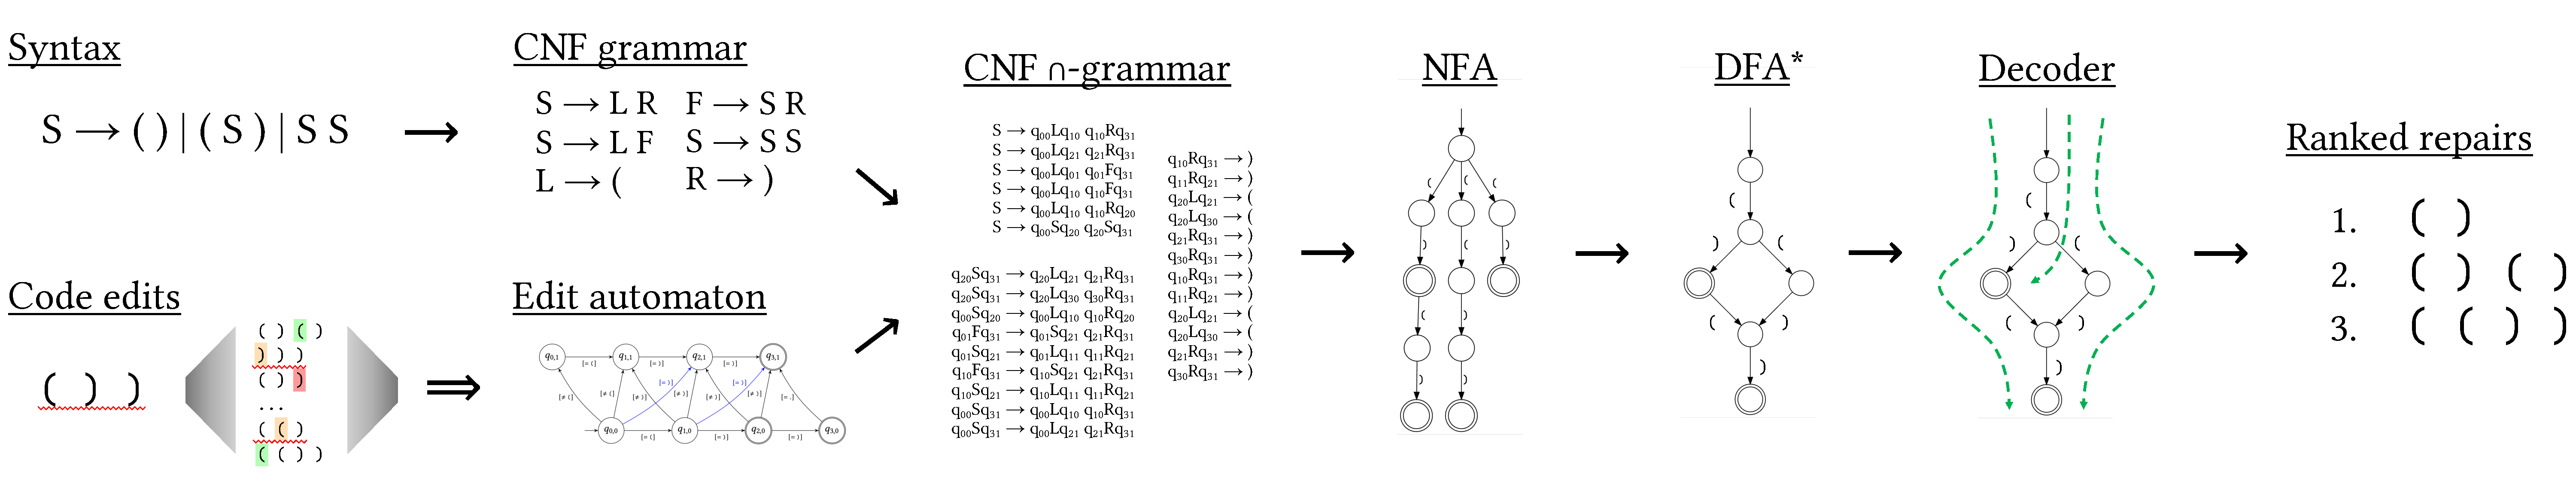
\includegraphics[width=\textwidth]{flow.pdf}\vspace{-1pt}
  \caption{Simplified dataflow. Given a grammar and broken code fragment, we create an automaton generating the language of small edits, then intersect it with the grammar to produce an intersection grammar, which can be simplified to a DFA and decoded.}\label{fig:arch_simp}
\end{figure}

To generate the repairs, we first construct an automaton that recognizes every string within a certain edit distance of the input. We then construct an intersection grammar, which recognizes all and only valid sequences within a certain edit distance of the input. This grammar is known to be non-recursive, and can be simplified to a deterministic finite automaton (DFA) using standard techniques. Finally, we decode the DFA to produce a list of repair candidates, which we rank by negative log likelihood under the language model.

Now that we have a high-level overview of our approach, we will give a demonstrate of some of the capabilities of our tool.

\section{Usage examples}

Tidyparse offers a user interface featuring a text editor, a grammar editor and a parse tree viewer for interactive prototyping. For example, suppose we have the following context-free grammar:

\begin{wholetidyinput}
  S -> S and S | S xor S | ( S ) | true | false | ! S(*@\caret{ }@*)
\end{wholetidyinput}

\noindent This grammar will automatically be rewritten into Chomsky Normal Form:

\begin{wholetidyinput}
 F.! (*@$\rightarrow$@*) !        S.) (*@$\rightarrow$@*) S F.)     and.S (*@$\rightarrow$@*) F.and S
F.( (*@$\rightarrow$@*) (      F.xor (*@$\rightarrow$@*) xor       xor.S (*@$\rightarrow$@*) F.xor S
F.) (*@$\rightarrow$@*) )      F.and (*@$\rightarrow$@*) and           S (*@$\rightarrow$@*) S xor.S
  S (*@$\rightarrow$@*) <S>        S (*@$\rightarrow$@*) false         S (*@$\rightarrow$@*) true
  S (*@$\rightarrow$@*) F.! S      S (*@$\rightarrow$@*) F.( S.)       S (*@$\rightarrow$@*) S and.S
  S (*@$\rightarrow$@*) S (*@$\varepsilon$@*)+      (*@$\varepsilon$@*)+ (*@$\rightarrow$@*) (*@$\varepsilon$@*)+ (*@$\varepsilon$@*)+         (*@$\varepsilon$@*)+ (*@$\rightarrow$@*) (*@$\varepsilon$@*)
\end{wholetidyinput}

%\noindent We can visualize the CFG as either a graph or a matrix:
%
%\begin{figure}[H]
%    
\includegraphics[width=3.5cm]{../figures/bool_arith_cfg_graph.png}
%    \hspace{20pt}
%    \includegraphics[width=3.5cm]{../figures/bool_arith_cfg_mat.bmp}
%\end{figure}

\noindent Given a string containing holes, our tool will return several completions in a few milliseconds:

\begin{tcolorbox}[left skip=0.7cm,
top=0.1cm,
middle=0mm,
boxsep=0mm,
underlay unbroken and first={%
  \path[draw=none] (interior.north west) rectangle node[white]{
\includegraphics[width=4mm]{../figures/tidyparse_logo.png}} ([xshift=-10mm,yshift=-9mm]interior.north west);
}]
\begin{lstlisting} [language=tidy, basicstyle=\ttfamily\small, escapeinside={(*@}{@*)}]
true _ _ _ ( false _ ( _ _ _ _ ! _ _ ) _ _ _ _(*@\caret{ }@*)
\end{lstlisting}
\tcblower
\begin{lstlisting} [language=tidy, basicstyle=\ttfamily\small, escapeinside={(*@}{@*)}]
1. true (*@\hlorange{xor}@*) (*@\hlorange{!}@*) ( false (*@\hlorange{xor}@*) ( (*@\hlorange{<S>}@*) (*@\hlorange{)}@*) (*@\hlorange{or}@*) ! (*@\hlorange{<S>}@*) ) (*@\hlorange{xor}@*) (*@\hlorange{<S>}@*)
2. true (*@\hlorange{xor}@*) (*@\hlorange{!}@*) ( false (*@\hlorange{and}@*) ( (*@\hlorange{<S>}@*) (*@\hlorange{)}@*) (*@\hlorange{or}@*) ! (*@\hlorange{<S>}@*) ) (*@\hlorange{xor}@*) (*@\hlorange{<S>}@*)
3. true (*@\hlorange{xor}@*) (*@\hlorange{!}@*) ( false (*@\hlorange{and}@*) ( (*@\hlorange{<S>}@*) (*@\hlorange{)}@*) (*@\hlorange{and}@*) ! (*@\hlorange{<S>}@*) ) (*@\hlorange{xor}@*) (*@\hlorange{<S>}@*)
4. true (*@\hlorange{xor}@*) (*@\hlorange{!}@*) ( false (*@\hlorange{and}@*) ( (*@\hlorange{<S>}@*) (*@\hlorange{)}@*) (*@\hlorange{and}@*) ! (*@\hlorange{<S>}@*) ) (*@\hlorange{and}@*) (*@\hlorange{<S>}@*)
...
\end{lstlisting}
\end{tcolorbox}

\noindent Similarly, if provided with a string containing various errors, it will return several suggestions how to fix it, where \hlgreen{green} is insertion, \hlorange{orange} is substitution and \hlred{red} is deletion.

\begin{tcolorbox}[left skip=0.7cm,
top=0.1cm,
middle=0mm,
boxsep=0mm,
underlay unbroken and first={%
  \path[draw=none] (interior.north west) rectangle node[white]{
\includegraphics[width=4mm]{../figures/tidyparse_logo.png}} ([xshift=-10mm,yshift=-9mm]interior.north west);
}]
\begin{lstlisting} [language=tidy, basicstyle=\ttfamily\small, escapeinside={(*@}{@*)}]
true and ( false or and true false(*@\caret{ }@*)
\end{lstlisting}
\tcblower
\begin{lstlisting} [language=tidy, basicstyle=\ttfamily\small, escapeinside={(*@}{@*)}]
1. true and ( false or (*@\hlorange{!}@*) true (*@\hlorange{)}@*)
2. true and ( false or (*@\hlgreen{<S>}@*) and true (*@\hlorange{)}@*)
3. true and ( false or (*@\hlorange{(}@*) true (*@\hlorange{)}@*) (*@\hlgreen{)}@*)
...
9. true and ( false or (*@\hlgreen{!}@*) (*@\hlgreen{<S>}@*) (*@\hlgreen{)}@*) and true (*@\hlred{false} @*)
\end{lstlisting}
\end{tcolorbox}

%Since CFLs are closed under homomorphisms, it is possible to unify lexing and parsing, however most languages explicitly define a separate lexer, which we avail to substitute named identifiers with their type. Given an invalid string, the tool will first abstract the raw characters, generate edits in the abstract token space, then remap successful repairs back to character space as shown below:
%
%\hspace{-0.4cm}\begin{minipage}[t]{0.485\textwidth}
%                 \begin{tcolorbox}[
%                 left skip=0.7cm,
%                 left=0.35cm,
%                 right=0cm,
%                 top=0.1cm,
%                 middle=0mm,
%                 boxsep=0mm,
%                 underlay unbroken and first={%
%                   \path[draw=none] (interior.north west) rectangle node[white]{
\includegraphics[width=4mm]{../figures/tidyparse_logo.png}} ([xshift=-10mm,yshift=-9mm]interior.north west);
%                 }]
%                 \begin{lstlisting} [hbox, language=tidy, basicstyle=\ttfamily\small, escapeinside={(*@}{@*)}]
%d = sum([foo(i] for i in vals))(*@\caret{ }@*)
%                 \end{lstlisting}
%                 \tcblower
%                 \begin{lstlisting} [hbox, language=tidy, basicstyle=\ttfamily\small, escapeinside={(*@}{@*)}]
%1. d = sum([foo(i(*@\hlorange{)}@*) for i in vals(*@\hlorange{]}@*))
%2. d = sum([(i(*@\hlorange{)}@*) for i in vals(*@\hlorange{]}@*))
%3. d = sum([foo(*@\hlorange{.}@*)i for i in vals(*@\hlorange{]}@*))
%4. d = sum([foo((*@\hlgreen{+}@*)i(*@\hlorange{)}@*) for i in vals(*@\hlorange{]}@*))
%                 \end{lstlisting}
%                 \end{tcolorbox}
%\end{minipage}
%\hspace{0.05cm}
%\begin{minipage}[t]{0.51\textwidth}
%  \begin{tcolorbox}[
%  left skip=0.7cm,
%  left=0.35cm,
%  right=0cm,
%  top=0.1cm,
%  middle=0mm,
%  boxsep=0mm,
%  underlay unbroken and first={%
%    \path[draw=none] (interior.north west) rectangle node[white]{
\includegraphics[width=4mm]{../figures/tidyparse_logo.png}} ([xshift=-10mm,yshift=-9mm]interior.north west);
%  }]
%  \begin{lstlisting} [language=tidy, basicstyle=\ttfamily\small, escapeinside={(*@}{@*)}]
%w = w ( [ w ( w ] for w in w ) )
%  \end{lstlisting}
%  \tcblower
%  \begin{lstlisting} [language=tidy, basicstyle=\ttfamily\small, escapeinside={(*@}{@*)}]
%1. w = w ( [ w ( i (*@\hlorange{)}@*) for i in w (*@\hlorange{]}@*) )
%2. w = w ( [ (*@\hlred{w}@*) ( w (*@\hlorange{)}@*) for w in w (*@\hlorange{]}@*) )
%3. w = w ( [ w (*@\hlorange{.}@*) w (*@\hlred{)}@*)  for w in w (*@\hlorange{]}@*) )
%4. w = w ( [ w ( (*@\hlgreen{+}@*) w (*@\hlorange{)}@*) for w in w (*@\hlorange{)}@*) )
%  \end{lstlisting}
%  \end{tcolorbox}
%\end{minipage}

For simplicity, it is also possible to define a grammar and string side-by-side, as shown in the untyped $\lambda$-calculus example below:

\begin{tcolorbox}[left skip=0.7cm,
top=0.1cm,
middle=0mm,
boxsep=0mm,
underlay unbroken and first={%
  \path[draw=none] (interior.north west) rectangle node[white]{
\includegraphics[width=4mm]{../figures/tidyparse_logo.png}} ([xshift=-10mm,yshift=-9mm]interior.north west);
}]
\begin{lstlisting} [language=tidy, basicstyle=\ttfamily\small, escapeinside={(*@}{@*)}]
sxp -> (*@$\lambda$@*) var . sxp | sxp sxp | var | ( sxp )
var -> a | b | c | f | x | y | z
---
( (*@$\lambda$@*) f . ( (*@$\lambda$@*) x . f ( x x ) ) ( (*@$\lambda$@*) x . f ( x x ) (*@\caret{ }@*)
\end{lstlisting}
\tcblower
\begin{lstlisting} [language=tidy, basicstyle=\ttfamily\small, escapeinside={(*@}{@*)}]
1. ( (*@$\lambda$@*) f . ( (*@$\lambda$@*) x . f ( x x ) ) (*@\hlorange{)}@*) (*@$\lambda$@*) x . f ( x x )
2. ( (*@$\lambda$@*) f . ( (*@$\lambda$@*) x . f ( x x ) ) (*@\hlorange{x}@*) (*@\hlgreen{)}@*) (*@$\lambda$@*) x . f ( x x )
3. ( (*@$\lambda$@*) f . ( (*@$\lambda$@*) x . f ( x x ) ) ( (*@$\lambda$@*) x . f ( x(*@\hlred{ }@*)) (*@\hlgreen{)}@*) (*@\hlgreen{)}@*)
\end{lstlisting}
\end{tcolorbox}

\noindent Name resolution and scope checking is also possible but requires a more sophisticated grammar.


\subsection{Grammar assistance}

Tidyparse uses a CFG to parse the CFG, so it can provide editing assistance while the user is designing the CFG. For example, if the CFG does not parse, will suggest a list of possible fixes.% In the future, we intend to use this functionality to perform example-based codesign and grammar induction.

  \begin{tcolorbox}[
  left skip=0.7cm,
  left=0.35cm,
  right=0cm,
  top=0.1cm,
  middle=0mm,
  boxsep=0mm,
  underlay unbroken and first={%
    \path[draw=none] (interior.north west) rectangle node[white]{
\includegraphics[width=4mm]{../figures/tidyparse_logo.png}} ([xshift=-10mm,yshift=-9mm]interior.north west);
  }]
  \begin{lstlisting} [language=tidy, basicstyle=\ttfamily\small, escapeinside={(*@}{@*)}]
B ::= true | false | (*@\caret{ }@*)
  \end{lstlisting}
  \tcblower
  \begin{lstlisting} [language=tidy, basicstyle=\ttfamily\small, escapeinside={(*@}{@*)}]
1. B (*@\hlorange{->}@*) true | false (*@\hlred{ }@*)
2. B (*@\hlorange{->}@*) true | false (*@\hlorange{<RHS>}@*)
3. B (*@\hlorange{->}@*) true | false | (*@\hlgreen{<RHS>}@*)
  \end{lstlisting}
  \end{tcolorbox}

\subsection{Interactive nonterminal expansion}

Users can interactively build up a complex expression by placing the caret over a nonterminal they wish to expand, then pressing \keys{\ctrl + \SPACE} to receive a list of possible substitutions.

\begin{tcolorbox}[left skip=0.7cm,
top=0.1cm,
middle=0mm,
boxsep=0mm,
underlay unbroken and first={%
  \path[draw=none] (interior.north west) rectangle node[white]{
\includegraphics[width=4mm]{../figures/tidyparse_logo.png}} ([xshift=-10mm,yshift=-9mm]interior.north west);
}]
\begin{lstlisting} [language=tidy, basicstyle=\ttfamily\small, escapeinside={(*@}{@*)}]
true and ( false or <(*@\caret{S}@*)> and true )
\end{lstlisting}
\tcblower
\begin{lstlisting} [language=tidy, basicstyle=\ttfamily\small, escapeinside={(*@}{@*)}]
1. true and ( false or (*@\hlorange{true}@*) and true )
2. true and ( false or (*@\hlorange{false}@*) and true )
3. true and ( false or (*@\hlorange{! <S>}@*) and true )
\end{lstlisting}
\end{tcolorbox}

\subsection{Nonterminal stubs}

Tidyparse augments CFGs with two additional rules, which are desugared into a vanilla CFG before parsing. The first rule, $\alpha\textsc{-sub}$, allows the user to define a nonterminal parameterized by $\alpha$, a non-recursive nonterminal in the same the CFG representing some finite type and its inhabitants. $\alpha\textsc{-sub}$ replaces all productions containing $\langle\alpha\rangle$ with the terminals in their transitive closure, $\alpha \rightarrow^* \beta$. The second rule, $\alpha\textsc{-int}$, introduces homonymous terminals for each user-defined nonterminal.

\begin{figure}[h!]
  \begin{prooftree}
    \AxiomC{$\mathcal{G} \vdash (w\langle\alpha\rangle \rightarrow x z) \in P$}
    \AxiomC{$\alpha^* : \{\beta \mid (\alpha \rightarrow^* \beta) \in P\}$}
    \RightLabel{$\alpha\textsc{-sub}$}
    \BinaryInfC{$\mathcal{G} \vdash \forall \beta \in \alpha^*.(w\langle\alpha\rangle \rightarrow x z)[\beta/\alpha] \in P'$}
  \end{prooftree}
  \begin{prooftree}
    \AxiomC{$\mathcal{G} \vdash v \in V$}
    \RightLabel{$\langle\cdot\rangle\textsc{-int}$}
    \UnaryInfC{$\mathcal{G} \vdash (v \rightarrow \langle v\rangle) \in P$}
  \end{prooftree}
\end{figure}

Tidyparse can also perform a limited form of type checking. Typed expressions are automatically expanded into ordinary nonterminals using the $\alpha\textsc{-sub}$ rule, for example when parsing an expression of the form $x + y$, the grammar will recognize \texttt{true + false} and \texttt{1 + 2}, but not \texttt{1 + true}.

\begin{tcolorbox}[left skip=0.7cm,
top=0.1cm,
middle=0mm,
boxsep=0mm,
underlay unbroken and first={%
  \path[draw=none] (interior.north west) rectangle node[white]{
\includegraphics[width=4mm]{../figures/tidyparse_logo.png}} ([xshift=-10mm,yshift=-9mm]interior.north west);
}]
\begin{lstlisting} [language=tidy, basicstyle=\ttfamily\small, escapeinside={(*@}{@*)}]
E<X> -> E<X> + E<X> | E<X> * E<X> | ( E<X> )
X -> Int | Bool
\end{lstlisting}
\tcblower
\begin{lstlisting} [language=tidy, basicstyle=\ttfamily\small, escapeinside={(*@}{@*)}]
E<Int> -> E<Int> + E<Int> | E<Int> * E<Int>
E<Bool> -> E<Bool> + E<Bool> | E<Bool> * E<Bool>
\end{lstlisting}
\end{tcolorbox}

\subsection{Syntax highlighting}

Subsequences which can be partly parseable are underlined in blue. Unparsable alphabetic tokens are marked orange. All other tokens are marked red.

\begin{tcolorbox}[left skip=0.7cm,
top=0.1cm,
middle=0mm,
boxsep=0mm,
underlay unbroken and first={%
  \path[draw=none] (interior.north west) rectangle node[white]{
\includegraphics[width=4mm]{../figures/tidyparse_logo.png}} ([xshift=-10mm,yshift=-9mm]interior.north west);
}]
\begin{lstlisting} [language=tidy, basicstyle=\ttfamily\small, escapeinside={(*@}{@*)}]
(*@\erb{( true xor false ) and true}@*) (*@\ero{xor}@*) (*@\ero{and}@*) (*@\err{not}@*) (*@\ero{false}@*)
\end{lstlisting}
\end{tcolorbox}
\end{document}